% Template for Cogsci submission with R Markdown

% Stuff changed from original Markdown PLOS Template
\documentclass[10pt, letterpaper]{article}

\usepackage{cogsci}
\usepackage{pslatex}
\usepackage{float}
\usepackage{caption}

% amsmath package, useful for mathematical formulas
\usepackage{amsmath}

% amssymb package, useful for mathematical symbols
\usepackage{amssymb}

% hyperref package, useful for hyperlinks
\usepackage{hyperref}

% graphicx package, useful for including eps and pdf graphics
% include graphics with the command \includegraphics
\usepackage{graphicx}

% Sweave(-like)
\usepackage{fancyvrb}
\DefineVerbatimEnvironment{Sinput}{Verbatim}{fontshape=sl}
\DefineVerbatimEnvironment{Soutput}{Verbatim}{}
\DefineVerbatimEnvironment{Scode}{Verbatim}{fontshape=sl}
\newenvironment{Schunk}{}{}
\DefineVerbatimEnvironment{Code}{Verbatim}{}
\DefineVerbatimEnvironment{CodeInput}{Verbatim}{fontshape=sl}
\DefineVerbatimEnvironment{CodeOutput}{Verbatim}{}
\newenvironment{CodeChunk}{}{}

% cite package, to clean up citations in the main text. Do not remove.
\usepackage{apacite}

% KM added 1/4/18 to allow control of blind submission
\cogscifinalcopy

\usepackage{color}

% Use doublespacing - comment out for single spacing
%\usepackage{setspace}
%\doublespacing


% % Text layout
% \topmargin 0.0cm
% \oddsidemargin 0.5cm
% \evensidemargin 0.5cm
% \textwidth 16cm
% \textheight 21cm

\title{Familiarity preference something something???}


\author{Gal Raz$^1$ (galraz@mit.edu), \bf{Anjie Cao$^2$  (anjiecao@stanford.edu)},\\ \bf{Michael C. Frank$^2$ (mcfrank@stanford.edu)},
 and \bf{Rebecca Saxe$^1$ (saxe@mit.edu)} \\
$^1$Department of Brain and Cognitive Sciences, MIT, $^2$Department of Psychology, Stanford University \\ }


\begin{document}

\maketitle

\begin{abstract}
haha

\textbf{Keywords:}
decision making; learning; bayesian modeling; cognitive development
\end{abstract}

\hypertarget{introduction}{%
\section{Introduction}\label{introduction}}

\hypertarget{experiment-1}{%
\section{Experiment 1}\label{experiment-1}}

\hypertarget{methods}{%
\subsection{Methods}\label{methods}}

\hypertarget{participants}{%
\subsection{Participants}\label{participants}}

66 children completed a task modified from the adult self-paced looking
time studies reported in CITE. Following our pre-registration (LINK), 2
children were excluded from the analysis because their performance in
the attention-check task failed to meet the inclusion criteria. We also
excluded trials with looking time that were three absolute deviations
away from the median in the log-transformed space across participants.
The final datasets includes 64 children in total (3YO: N = 18; 4YO: N =
26; 5YO: N = 20). All participants were recruited in a
university-affiliated research preschool.

\hypertarget{stimuli}{%
\subsection{Stimuli}\label{stimuli}}

We used a subset of stimuli created for the adult self-paced looking
time studies. In the previous study, we created a set of animated
creatures using Spore (a game developed by Maxis in 2008). Half of the
creatures had high perceptual complexity, and half had low perceptual
complexity. We used the high perceptual complexity stimuli for the
current study.

\hypertarget{procedures}{%
\subsection{Procedures}\label{procedures}}

Children were tested individually in a test room by an experimenter. The
experimenter invited the child to ``meet some monster friends'' and then
familiarized the child with the laptop computer used to present the
experiment. Before the test, each child went through a practice phase
where they practiced pressing the space bar to move on to the next
trial. The child was instructed that they can press the key and move on
to meet more monster friends whenever they want.

On each trial, the child would see an animated creature appear on the
screen. The child can move on to the next trial by pressing the space
bar. Each block consisted of six trials. Usually, the same creature will
be shown repeatedly (the background stimulus), but each block could
contain either zero or one deviant trial. Deviant trials were trials
that present a different creature from the background stimulus. Deviant
trials appeared on the second, the fourth, or the sixth trial of the
block. Each child saw eight blocks in total.

At the offset of each block, a memory task was presented to ensure
children are appropriately attending to the task. The memory task was a
2-Alternative Forced Choice (2AFC) question, asking the children to
identify which of the two stimuli they have seen before. The pair of
stimuli contained one stimulus used as a background stimulus in the
preceding block and a novel stimulus that did not appear anywhere else
in the experiment.

\hypertarget{results-and-discussion}{%
\subsection{Results and discussion}\label{results-and-discussion}}

\begin{CodeChunk}

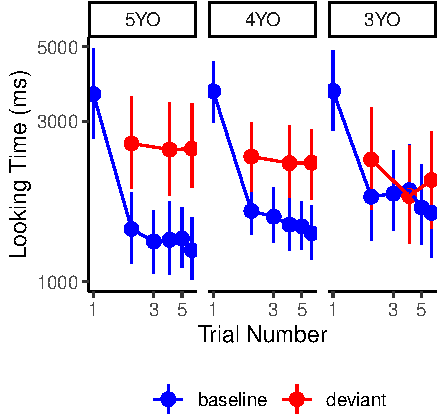
\includegraphics{figs/unnamed-chunk-10-1} \end{CodeChunk}

We anticipated that the preschooler children would show patterns of
habituation and dishabituation similar to adults. We also expected to
see developmental changes in the shape of habituation trajectories. Our
pre-registered mixed-effect mod includes a three-way interaction term
between age (in months; scaled and centered), trial number, and trial
type (background or deviant) to predict log-transformed looking time.
The interaction between the trial number and trial type was significant,
suggesting the paradigm has captured habituation and novelty preference
in preschoolers (\(\beta\) = 0.14, \emph{SE} = 0.02, \emph{t} = 6.22,
\emph{p} \textless{} 0.01). However, we did not find any significant
interaction with age, nor was the main effect significant (all \emph{p}
\textgreater{} 0.1).

We also explored the potential familiarity preference by comparing the
looking time at the second background trial and the second deviant
trial. Under the Hunter \& Ames (1988), the second trial in each block
is most likely to yield a familiarity preference, since participants
receivee the least amount of familiarization with the background
stimulus in a block. If there was a familiarity preference, participants
should look longer at a background trial than a deviant trial. However,
we did not find evidence supporting this prediction. We ran a mixed
effect model predicting looking time at the second trial with trial type
as the predictor. There was a significant trial type effect in the
opposite direction, suggesting participants looked longer at the deviant
trial than the background trial even with as little as one trial of
familiarization time (\(\beta\) = 0.41, \emph{SE} = 0.03, \emph{t} =
12.24, \emph{p} \textless{} 0.01).

In summary, this experiment captured habituation and novelty preference
with in preschoolers, replicating the patterns we saw in the previous
adult samples (CITE). Notably, under the current paradigm, we did not
find any evidence of familiarity preference. We moved to the infant
samples in the next experiment.

\hypertarget{experiment-2}{%
\section{Experiment 2}\label{experiment-2}}

\hypertarget{methods-1}{%
\subsection{Methods}\label{methods-1}}

\hypertarget{results-and-discussion-1}{%
\subsection{Results and discussion}\label{results-and-discussion-1}}

\hypertarget{cache-pre-registered-models}{%
\section{cache pre-registered
models}\label{cache-pre-registered-models}}

\(\beta\) = \texttt{r}; \emph{SE} = \texttt{r}; \emph{t} = \texttt{r};
\emph{p} = \texttt{r}

To test the prediction that partial encoding elicits familiarity
preferences, while complete encoding elicits novelty preferences, we
pre-registered a model which allows for a non-linear interaction between
exposure duration by adding a quadratic effect of familiarization
duration, and its interaction with novelty.

We found that neither the main effect, nor the interaction of that
quadratic term were significant (Main effect: \(\beta\) = 0.46;
\emph{SE} = 0.88; \emph{t} = 0.53; \emph{p} = 0.6; Interaction effect:
\(\beta\) = 0.4; \emph{SE} = 1.58; \emph{t} = 0.26; \emph{p} = 0.8),
while the interaction of novelty with the linear term was significant
(\(\beta\) = 4.38; \emph{SE} = 1.56; \emph{t} = 2.8; \emph{p} = 0.01).
This suggests that novelty preferences get stronger as a function
familiarization duration, but that there is no special effect of partial
encoding as posited by H\&A. Furthermore, there was a significant
decrease in looking times to the familiar items as a function of
familiarization duration, indicating that infants habituated to familiar
stimuli in our paradigm (\(\beta\) = -2.32; \emph{SE} = 0.87; \emph{t} =
-2.66; \emph{p} = 0.01).

We next tested specifically for the existence of familiarity preference
in our dataset. After finding a hint of a familiarity preference after
four familiarizations in the first study, which did not turn out
significant in an exploratory analysis (\(\beta\) = -0.2; \emph{SE} = ;
\emph{t} = -1.06; \emph{p} = 0.3), we argued that if familiarity
preferences are driven by partial encoding, any condition in which there
were fewer exposures should also reveal a familiarity preference. We
therefore tested whether looking to the familiar stimulus was longer in
all trial with four or less exposures, which it did not (\(\beta\) =
0.07; \emph{SE} = ; \emph{t} = 0.65; \emph{p} = 0.52).

Novelty preferences, on the other hand, were robust after 8 (\(\beta\) =
0.5; \emph{SE} = ; \emph{t} = 2.9; \emph{p} = 0.01) and 9
familiarizations (\(\beta\) = 0.6; \emph{SE} = ; \emph{t} = 4.15;
\emph{p} \textless{} 0.01), as well as in the combined dataset
(\(\beta\) = 0.54; \emph{SE} = ; \emph{t} = 4.44; \emph{p} \textless{}
0.01).

\hypertarget{general-discussion}{%
\section{General discussion}\label{general-discussion}}

\hypertarget{references}{%
\section{References}\label{references}}

\setlength{\parindent}{-0.1in} 
\setlength{\leftskip}{0.125in}

\noindent

\bibliographystyle{apacite}


\end{document}
